\documentclass{article}

  % packages
    % basic stuff for rendering math
    \usepackage[letterpaper, top=1in, bottom=1in, left=1in, right=1in]{geometry}
    \usepackage[utf8]{inputenc}
    \usepackage[english]{babel}
    \usepackage{amsmath} 
    \usepackage{amssymb}

    % extra math symbols and utilities
    \usepackage{mathtools}        % for extra stuff like \coloneqq
    \usepackage{mathrsfs}         % for extra stuff like \mathsrc{}
    \usepackage{centernot}        % for the centernot arrow 
    \usepackage{bm}               % for better boldsymbol/mathbf 
    \usepackage{enumitem}         % better control over enumerate, itemize
    \usepackage{hyperref}         % for hypertext linking
    \usepackage{xr-hyper}
    \usepackage{fancyvrb}          % for better verbatim environments
    \usepackage{newverbs}         % for texttt{}
    \usepackage{xcolor}           % for colored text 
    \usepackage{listings}         % to include code
    \usepackage{lstautogobble}    % helper package for code
    \usepackage{parcolumns}       % for side by side columns for two column code
    

    % page layout
    \usepackage{fancyhdr}         % for headers and footers 
    \usepackage{lastpage}         % to include last page number in footer 
    \usepackage{parskip}          % for no indentation and space between paragraphs    
    \usepackage[T1]{fontenc}      % to include \textbackslash
    \usepackage{footnote}
    \usepackage{etoolbox}

    % for custom environments
    \usepackage{tcolorbox}        % for better colored boxes in custom environments
    \tcbuselibrary{breakable}     % to allow tcolorboxes to break across pages

    % figures
    \usepackage{pgfplots}
    \pgfplotsset{compat=1.18}
    \usepackage{float}            % for [H] figure placement
    \usepackage{tikz}
    \usepackage{tikz-cd}
    \usepackage{circuitikz}
    \usetikzlibrary{arrows}
    \usetikzlibrary{positioning}
    \usetikzlibrary{calc}
    \usepackage{graphicx}
    \usepackage{algorithm, algpseudocode}
    \usepackage{caption} 
    \usepackage{subcaption}
    \captionsetup{font=small}

    % for tabular stuff 
    \usepackage{dcolumn}

    \usepackage[nottoc]{tocbibind}
    \pdfsuppresswarningpagegroup=1
    \hfuzz=5.002pt                % ignore overfull hbox badness warnings below this limit

  % New and replaced operators
    \DeclareMathOperator{\Tr}{Tr}
    \DeclareMathOperator{\Sym}{Sym}
    \DeclareMathOperator{\Span}{span}
    \DeclareMathOperator{\std}{std}
    \DeclareMathOperator{\Cov}{Cov}
    \DeclareMathOperator{\Var}{Var}
    \DeclareMathOperator{\Corr}{Corr}
    \DeclareMathOperator{\prox}{prox}
    \DeclareMathOperator{\pos}{pos}
    \DeclareMathOperator*{\argmin}{\arg\!\min}
    \DeclareMathOperator*{\argmax}{\arg\!\max}
    \newcommand{\ket}[1]{\ensuremath{\left|#1\right\rangle}}
    \newcommand{\bra}[1]{\ensuremath{\left\langle#1\right|}}
    \newcommand{\braket}[2]{\langle #1 | #2 \rangle}
    \newcommand{\qed}{\hfill$\blacksquare$}     % I like QED squares to be black

  % Custom Environments
    \newtcolorbox[auto counter, number within=section]{question}[1][]
    {
      colframe = orange!25,
      colback  = orange!10,
      coltitle = orange!20!black,  
      breakable, 
      title = \textbf{Question \thetcbcounter ~(#1)}
    }

    \newtcolorbox[auto counter, number within=section]{exercise}[1][]
    {
      colframe = teal!25,
      colback  = teal!10,
      coltitle = teal!20!black,  
      breakable, 
      title = \textbf{Exercise \thetcbcounter ~(#1)}
    }
    \newtcolorbox[auto counter, number within=section]{solution}[1][]
    {
      colframe = violet!25,
      colback  = violet!10,
      coltitle = violet!20!black,  
      breakable, 
      title = \textbf{Solution \thetcbcounter}
    }
    \newtcolorbox[auto counter, number within=section]{lemma}[1][]
    {
      colframe = red!25,
      colback  = red!10,
      coltitle = red!20!black,  
      breakable, 
      title = \textbf{Lemma \thetcbcounter ~(#1)}
    }
    \newtcolorbox[auto counter, number within=section]{theorem}[1][]
    {
      colframe = red!25,
      colback  = red!10,
      coltitle = red!20!black,  
      breakable, 
      title = \textbf{Theorem \thetcbcounter ~(#1)}
    } 
    \newtcolorbox[auto counter, number within=section]{proposition}[1][]
    {
      colframe = red!25,
      colback  = red!10,
      coltitle = red!20!black,  
      breakable, 
      title = \textbf{Proposition \thetcbcounter ~(#1)}
    } 
    \newtcolorbox[auto counter, number within=section]{corollary}[1][]
    {
      colframe = red!25,
      colback  = red!10,
      coltitle = red!20!black,  
      breakable, 
      title = \textbf{Corollary \thetcbcounter ~(#1)}
    } 
    \newtcolorbox[auto counter, number within=section]{heuristic}[1][]
    {
      colframe = red!25,
      colback  = red!10,
      coltitle = red!20!black,  
      breakable, 
      title = \textbf{Heuristic \thetcbcounter ~(#1)}
    } 
    \newtcolorbox[auto counter, number within=section]{proof}[1][]
    {
      colframe = orange!25,
      colback  = orange!10,
      coltitle = orange!20!black,  
      breakable, 
      title = \textbf{Proof. }
    } 
    \newtcolorbox[auto counter, number within=section]{definition}[1][]
    {
      colframe = yellow!25,
      colback  = yellow!10,
      coltitle = yellow!20!black,  
      breakable, 
      title = \textbf{Definition \thetcbcounter ~(#1)}
    } 
    \newtcolorbox[auto counter, number within=section]{example}[1][]
    {
      colframe = blue!25,
      colback  = blue!10,
      coltitle = blue!20!black,  
      breakable, 
      title = \textbf{Example \thetcbcounter ~(#1)}
    } 
    \newtcolorbox[auto counter, number within=section]{code}[1][]
    {
      colframe = green!25,
      colback  = green!10,
      coltitle = green!20!black,  
      breakable, 
      title = \textbf{Code \thetcbcounter ~(#1)}
    } 
    \newtcolorbox[auto counter, number within=section]{algo}[1][]
    {
      colframe = green!25,
      colback  = green!10,
      coltitle = green!20!black,  
      breakable, 
      title = \textbf{Algorithm \thetcbcounter ~(#1)}
    } 

    \definecolor{dkgreen}{rgb}{0,0.6,0}
    \definecolor{gray}{rgb}{0.5,0.5,0.5}
    \definecolor{mauve}{rgb}{0.58,0,0.82}
    \definecolor{darkblue}{rgb}{0,0,139}
    \definecolor{lightgray}{gray}{0.93}
    \renewcommand{\algorithmiccomment}[1]{\hfill$\triangleright$\textcolor{blue}{#1}}

    % default options for listings (for code)
    \lstset{
      autogobble,
      frame=ltbr,
      language=Python,
      aboveskip=3mm,
      belowskip=3mm,
      showstringspaces=false,
      columns=fullflexible,
      keepspaces=true,
      basicstyle={\small\ttfamily},
      numbers=left,
      firstnumber=1,                        % start line number at 1
      numberstyle=\tiny\color{gray},
      keywordstyle=\color{blue},
      commentstyle=\color{dkgreen},
      stringstyle=\color{mauve},
      backgroundcolor=\color{lightgray}, 
      breaklines=true,                      % break lines
      breakatwhitespace=true,
      tabsize=3, 
      xleftmargin=2em, 
      framexleftmargin=1.5em, 
      stepnumber=1
    }

  % Page style
    \pagestyle{fancy}
    \fancyhead[L]{Optimization}
    \fancyhead[C]{Muchang Bahng}
    \fancyhead[R]{Spring 2025} 
    \fancyfoot[C]{\thepage / \pageref{LastPage}}
    \renewcommand{\footrulewidth}{0.4pt}          % the footer line should be 0.4pt wide
    \renewcommand{\thispagestyle}[1]{}  % needed to include headers in title page

  % external documents 
  %  \externaldocument[place-]{../Machine_Learning/paper}[../Machine_Learning/paper.pdf] 

\begin{document}

\title{Optimization}
\author{Muchang Bahng}
\date{Spring 2025}

\maketitle
\tableofcontents
\pagebreak

This covers computability theory, complexity theory, and automata theory. 
Alphabet. Boolean logic

 
\section{Gradient Methods} 

  The first thing you learn about gradients in multivariate calculus is that they point in the step of steepest ascent. Therefore, 

\subsection{Newton-Raphson Method}


\subsection{Stochastic Gradient Descent} 

  Note that gradient computation is generally very expensive and not scalable as $n$ gets high. Given a dataset $\mathcal{D} = \{d_i\}_i$ of $D$ points, our posterior is of the form $p(\theta \mid \mathcal{D}) \propto p(\mathcal{D} \mid \theta) \, p(\theta)$ and so 
  \begin{equation}
    \nabla_\theta \log p(\theta \mid \mathcal{D}) = \nabla_\theta \log{p(\theta)} + \nabla_\theta \log{p(\mathcal{D} \mid \theta)} = \nabla_\theta \log{p(\theta)} + \sum_i \nabla_\theta \log{p(d_i \mid \theta)}
  \end{equation}

  We can approximate this gradient by taking a minibatch of $\mathcal{D}$. Let us take a minibatch of $m$ samples $M_m (\mathcal{D})$ without replacement, where $m << D$. Then, our approximation of the gradient of the log likelihood is 

  \begin{equation}
    \nabla_\theta \log{p(\mathcal{D} \mid \theta)} \approx \nabla_\theta \log{p (M_m (\mathcal{D}) \mid \theta)} \coloneqq \frac{D}{m} \sum_{d \in M_m(\mathcal{D})} \nabla_\theta \log{p(d \mid \theta)}
  \end{equation}

  and thus our noisy gradient approximation of the gradient of the log posterior is 

  \begin{equation}
    \nabla_\theta \log{p(\theta \mid \mathcal{D})} \approx \nabla_\theta \log{p(\theta \mid M_m(\mathcal{D}))} \coloneqq \nabla_\theta \log{p(\theta)} + \nabla_\theta \log{p (M_m (\mathcal{D}) \mid \theta)}
  \end{equation}

  The classical gradient ascent algorithm simply optimizes a concave function, or if $f$ is multimodal, finds a local maxima. When we use the entire $\mathcal{D}$ to compute the gradient, we call this a \textit{batch gradient descent}, and if the minibatch estimate of the gradient is used, then this is called \textit{stochastic gradient descent}. Ideally, we would want to have a variable step size $h(t)$ so that $h \rightarrow 0$ as $t \rightarrow + \infty$. 

  \begin{algorithm}
    \caption{Stochastic Gradient Ascent}\label{alg:sgd}
    \begin{algorithmic}

    \Require Initial $\boldsymbol{\theta}_0$, Stepsize function $h(t)$, Minibatch size $m$

    \For{$t = 0$ to $T$ until convergence,}
        \State $\hat{g}(\theta_t) \gets \nabla_\theta \log{p(\theta_t \mid M_m(\mathcal{D}))}$
        \State $\theta_{t+1} \gets \theta_t + h(t) \cdot \hat{g}(\theta_t)$
    \EndFor

    \end{algorithmic}
  \end{algorithm}

  SGD with momentum. 

  We have assumed knowledge of gradient descent in the back propagation step in the previous section, but let's revisit this by looking at linear regression. Given our dataset $\mathcal{D} = \{\mathbf{x}^(n), y^{(n)}\}$, we are fitting a linear model of the form 
  \begin{equation}
    f(\mathbf{x}; \mathbf{w}, b) = \mathbf{w}^T \mathbf{x} + b
  \end{equation} 
  The squared loss function is 
  \begin{equation}
    \mathcal{L}(\mathbf{w}, b) = \frac{1}{2} \sum_{n=1}^N \big( y - f(\mathbf{x}; \mathbf{w}, b) \big)^2 = \frac{1}{2} \sum_{n=1}^N \big( y - (\mathbf{w}^T \mathbf{x} + b) \big)^2  
  \end{equation}
  If we want to minimize this function, we can visualize it as a $d$-dimensional surface that we have to traverse. Recall from multivariate calculus that the gradient of an arbitrary function $\mathcal{L}$ points in the steepest direction in which $\mathcal{L}$ increases. Therefore, if we can compute the gradient of $\mathcal{L}$ and step in the \textit{opposite direction}, then we would make the more efficient progress towards minimizing this function (at least locally). The gradient can be solved using chain rule. Let us solve it with respect to $\mathbf{w}$ and $b$ separately first. Beginners might find it simpler to compute the gradient element-wise. 
  \begin{align}
    \frac{\partial}{\partial w_j} \mathcal{L}(\mathbf{w}, b) 
    & = \frac{\partial}{\partial w_j} \bigg(\frac{1}{2} \sum_{n=1}^N \Big( f (\mathbf{x}^{(n)}; \mathbf{w}, b) - y^{(n)} \Big)^2 \bigg) \\
    & = \frac{1}{2} \sum_{n=1}^N \frac{\partial}{\partial w_j} \Big( f(\mathbf{x}^{(n)}; \mathbf{w}, b) - y^{(n)}\Big)^2 \\
    & = \frac{1}{2} \sum_{n=1}^N 2 \Big( f(\mathbf{x}^{(n)}) - y^{(n)}\Big) \cdot \frac{\partial}{\partial w_j} \big( f(\mathbf{x}^{(n)}; \mathbf{w}, b) - y^{(n)} \big) \\
    & = \frac{1}{2} \sum_{n=1}^N 2 \Big( f(\mathbf{x}^{(n)}) - y^{(n)}\Big) \cdot \frac{\partial}{\partial w_j} \big( \mathbf{w}^T \mathbf{x}^{(n)} + b - y^{(n)} \big) \\
    & = \sum_{n=1}^N \big( f(\mathbf{x}^{(n)}; \mathbf{w}, b) - y^{(n)}\big) \cdot x_j^{(n)} \;\;\;\;\;(\text{for } j = 0, 1, \ldots, d)
  \end{align}
  As for getting the derivative w.r.t. $b$, we can redo the computation and get 
  \begin{equation}
    \frac{\partial}{\partial w_j}\mathcal{L}(\mathbf{w}, b) = \sum_{n=1}^N \big( f (\mathbf{x}^{(n)}; \mathbf{w}, b) - y^{(n)}\big) 
  \end{equation}
  and in the vector form, setting $\boldsymbol{\theta} = (\mathbf{w}, b)$, we can set 
  \begin{align}
    \nabla \mathcal{L} (\mathbf{w}) & = \mathbf{X}^T (\hat{\mathbf{y}} - \mathbf{y}) \\
    \nabla \mathcal{L} (b) & = (\hat{\mathbf{y}} - \mathbf{y}) \cdot \mathbf{1}
  \end{align}
  where $\hat{\mathbf{y}}_n = f(\mathbf{x}^{(n)}; \mathbf{w}, b)$ are the predictions under our current linear model and $\mathbf{X} \in \mathbb{R}^{n \times d}$ is our design matrix. This can easily be done on a computer using a package like \texttt{numpy}. Remember that GD is really just an algorithm that updates $\boldsymbol{\theta}$ repeatedly until convergence, but there are a few problems.
  \begin{enumerate}
    \item The algorithm can be susceptible to local minima. A few countermeasures include shuffling the training set or randomly choosing initial points $\theta$
    \item The algorithm may not converge if $\alpha$ (the step size) is too high, since it may overshoot. This can be solved by reducing the $\alpha$ with each step, using \textit{schedulers}. 
    \item The entire training set may be too big, and it may therefore be computationally expensive to update $\boldsymbol{\theta}$ as a whole, especially if $d >> 1$. This can be solved using stochastic gradient descent.
  \end{enumerate}

  Rather than updating the vector $\boldsymbol{\theta}$ in batches, we can apply \textbf{stochastic gradient descent} that works incrementally by updating $\boldsymbol{\theta}$ with each term in the summation. That is, rather than updating as a batch by performing the entire matrix computation by multiplying over $N$ dimensions,
  \begin{equation}
    \nabla \mathcal{L} (\mathbf{w}) = \underbrace{\mathbf{X}^T}_{D \times N} \underbrace{(\hat{\mathbf{y}} - \mathbf{y})}_{N \times 1}
  \end{equation}
  we can reduce this load by choosing a smaller subset $\mathcal{M} \subset \mathcal{D}$ of $M < N$ elements, which gives 
  \begin{equation}
    \nabla \mathcal{L}_{\mathcal{M}} (\mathbf{w}) = \underbrace{\mathbf{X}_{\mathcal{M}}^T}_{D \times M} \underbrace{(\hat{\mathbf{y}_{\mathcal{M}}} - \mathbf{y}}_{\mathcal{M}})_{M \times 1}
  \end{equation}
  The reason we can do this is because of the following fact.  
  
  \begin{theorem}[Unbiasedness of SGD]
    $\nabla \mathcal{L}_{\mathcal{M}} (\mathbf{w})$ is an \textit{unbiased estimator} of the true gradient. That is, setting $\mathcal{M}$ as a random variable of samples over $\mathcal{D}$, we have 
    \begin{equation}
      \mathbb{E}_{\mathcal{M}} [\nabla \mathcal{L}_{\mathcal{M}} (\mathbf{w})] = \nabla \mathcal{L} (\mathbf{w})
    \end{equation}
  \end{theorem}
  \begin{proof}
    We use linearity of expectation for all $\mathcal{M} \subset \mathcal{D}$ of size $M$. 
  \end{proof}

  Even though these estimators are noisy, we get to do much more iterations and therefore have a faster net rate of convergence. By using repeated chain rule, or a fancier term is automatic differentiation, as shown before, SGD can be used to optimize neural networks. 

  Extending beyond SGD, there are other optimizers we can use. Essentially, we are doing a highly nonconvex optimization, which doesn't have a straightforward answer, so the best we can do is play around with some properties. 0th order approximations are hopeless since the dimensions are too high, and second order approximations are hopeless either since computing the Hessian is too expensive for one run. Therefore, we must resort to some first order methods, which utilize the gradient. Some other properties to consider are: 
  \begin{enumerate} 
    \item Learning rate 
    \item Momentum 
    \item Batch Size
  \end{enumerate}

\subsection{Momentum and Nesterov}

\subsection{Block Coordinate Descent} 


\section{Subgradient Methods}

  \begin{definition}[Convex Function]
    A function $f: U \subset \mathbb{R}^n \rightarrow \mathbb{R}$ defined on a convex set $U$ is convex if and only if for any $\mathbf{x}, \mathbf{y} \in U$
    \begin{equation}
      f \big(\lambda \mathbf{x} + (1 - \lambda) \mathbf{y} \big) \leq \lambda f(\mathbf{x}) + (1 - \lambda) f(\mathbf{y})
    \end{equation}
    Now if $f$ is differentiable, then convexity is equivalent to 
    \begin{equation}
      f(x) \geq f(y) + \nabla f(y)^T \cdot (x - y)
    \end{equation}
    for all $x, y \in U$. That is, its local linear approximation always underestimates $f$. 
  \end{definition}

  It is well known that the mean square error of a linear map is convex. However, when we impose the L1 penalty, the loss function is now not differentiable at $\mathbf{0}$. Therefore, we must introduce the notion of a subgradient. 

  \begin{definition}[Subgradient]
    The subgradient of a convex function $f: U \subset \mathbb{R}^n \rightarrow \mathbb{R}$ is any linear map $\mathbf{A} (x): \mathbb{R}^n \rightarrow \mathbb{R}$ such that 
    \begin{equation}
      f(\mathbf{y}) \geq f(\mathbf{x}) + \mathbf{A}(\mathbf{x}) (\mathbf{y} - \mathbf{x})
    \end{equation}
    for any $\mathbf{y} \in U$. The set of all subgradients at $\mathbf{x}$ is called the \textbf{subdifferential} defined 
    \begin{equation}
      \partial f (\mathbf{x}) = \{ \mathbf{A} \in \mathbb{R}^n \mid \mathbf{A} \text{ is a subgradient of } f \text{ at } \mathbf{x} \}
    \end{equation}
  \end{definition}

  The subgradient also acts as a linear approximation of $f$, but now at nondifferentiable points of convex functions, we have a set of linear approximations. It is clear that the subgradient at a differentiable point is uniquely the gradient ($\partial f(\mathbf{x}) = \{ \nabla f(\mathbf{x})$), but for places like the absolute value, we can have infinite linear approximations. 
  \begin{center}
    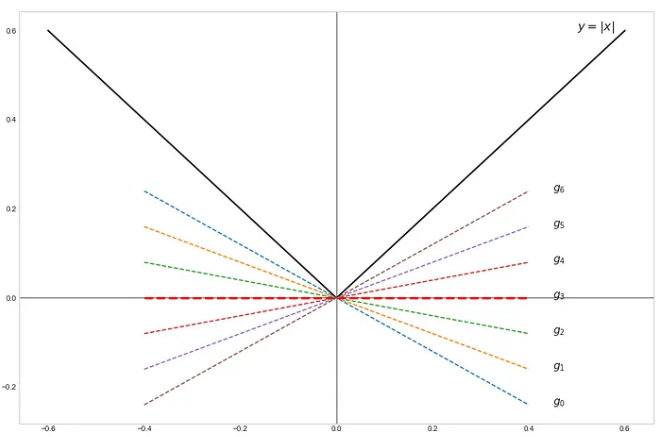
\includegraphics[scale=0.4]{img/subgradient_of_abs.png}
  \end{center}
  Given the subdifferential, thus the optimality condition for any convex $\mathbf{f}$ (differentiable or not) is
  \begin{equation}
    f(\mathbf{x}^\ast) = \min_{\mathbf{x}} f(\mathbf{x}) \iff \mathbf{0} \in \partial f(\mathbf{x}^\ast)
  \end{equation}
  known as the subgradient optimality condition, which clearly implies 
  \begin{equation}
    f(\mathbf{y}) \geq f(\mathbf{x}^\ast) + \mathbf{0}^T (\mathbf{y} - \mathbf{x}^\ast) = f(\mathbf{x}^\ast)
  \end{equation}

  \begin{example}
    The subdifferential of the absolute value function $f(x) = |x|$ at any given $x$ is 
    \begin{equation}
      \partial f(x) = \begin{cases} 1 & \text{ if } x > 0 \\ [-1, 1] & \text{ if } x = 0 \\ -1 & \text{ if } x < 0 \end{cases}
    \end{equation}
  \end{example}

\subsection{Proximal Gradient Descent}

  \begin{definition}[Proximal Operator]
    Given a lower semicontinuous convex function $f$ mapping from Hilbert space $X$ to $[-\infty, +\infty]$, its \textbf{proximal operator} associated with a point $u$ is defined 
    \begin{equation}
      \prox_{f, \tau} (u) = \argmin_{x} \bigg( f(x) + \frac{1}{2\tau} ||x - u||^2 \bigg)
    \end{equation}
    where $\tau > 0$ is a parameter that scales the quadratic term. This is basically the point that minimizes the sum of $f(x)$ and the square of the Euclidean distance between $x$ and $u$, scaled by $1/2\tau$. 
  \end{definition}

  Now given the loss function $L (\boldsymbol{\theta}) = L_{\mathrm{obj}} (\boldsymbol{\theta}) + L_{\mathrm{reg}} (\boldsymbol{\theta})$, we want to compute the proximal operator on the regularization loss and update that with the gradient of the smooth objective loss. 
  \begin{equation}
    \boldsymbol{\theta}^{(k+1)} = \prox_{L_{\mathrm{reg}}, \tau} \big[ \boldsymbol{\theta}^{(k)} - \tau \nabla L_{\mathrm{obj}} (\boldsymbol{\theta}^{(k)}) \big]
  \end{equation}
  Let's compute the proximal operator of the L1 loss $h(\boldsymbol{\theta}) = \lambda ||\boldsymbol{\theta}||_1$. We can parameterize this loss by the $\lambda$, so we will use the notation $\prox_{\lambda, \tau}$ rather than $\prox_{h, \tau}$. 
  \begin{align*}
    \prox_{\lambda, \tau} (\mathbf{u}) & = \argmin_{\boldsymbol{\theta}} \bigg( \lambda ||\boldsymbol{\theta}||_1 + \frac{1}{2\tau} ||\boldsymbol{\theta} - \mathbf{u}||_2^2 \bigg) \\
    & = \argmin_{\boldsymbol{\theta}} \bigg( \sum_{i=1}^n \lambda |\theta_i| + \frac{1}{2\tau} (\theta_i - u_i)^2 \bigg) 
  \end{align*}
  These are separable functions that can be decoupled and optimized component-wise. So, we really just want to find 
  \begin{equation}
    \theta_i^\ast = \argmin_{\theta_i} \bigg( \lambda |\theta_i| + \frac{1}{2\tau} (\theta_i - u_i)^2 \bigg)
  \end{equation}
  The sum of convex functions is convex, and so we should differentiate it and find where the gradient is $0$ to optimize it. 
  \begin{enumerate}
    \item When $\theta_i > 0$, then we minimize $\lambda \theta_i + \frac{1}{2\tau} (\theta_i - u_i)^2$, so taking the gradient and setting to $0$ gives 
    \begin{equation}
      \theta_i = u_i - \lambda \tau
    \end{equation}
    subject to the constraint that $\theta_i > 0$, or equivalently, that $u_i > \lambda \tau$. 

    \item When $\theta_i < 0$, then we minimize $-\lambda \theta_i + \frac{1}{2\tau} ( \theta_i - u_i)^2$, so taking the gradient and setting to $0$ gives 
    \begin{equation}
      \theta_i = u_i + \lambda \tau
    \end{equation}
    subject to the constraint that $\theta_i < 0$, or equivalently, that $u_i < -\lambda \tau$. 

    \item When $\theta_i = 0$, then we minimize $\lambda |\theta_i| + \frac{1}{2\tau} (\theta_i - u_i)^2$, which doesn't have derivative at $\theta_i = 0$. So, we can compute the subdifferential of it to get 
    \[0 \in \partial \bigg( \lambda |\theta_i| + \frac{1}{2\tau} (\theta_i - u_i)^2 \bigg) = \lambda \partial (|\theta_i|) + \frac{1}{\tau} (\theta_i - u_i)\]
    Now at $\theta_i = 0$, the subdifferential can be any value in $[-1, 1]$, and the above reduces to 
    \begin{equation}
      0 \in \lambda [-1, 1] - \frac{1}{\tau} u_i
    \end{equation}
    this is equivalent to saying that $u_i/\tau$ is contained in the interval $[-\lambda, \lambda]$, meaning that $u_i \in [-\lambda \tau, \lambda \tau]$. 
  \end{enumerate}

  Ultimately we get that 
  \begin{equation}
    \prox_{\lambda, \tau} (u) = \begin{cases} u - \lambda \tau & \text{ if } u > \lambda \tau \\ 0 & \text{ if } |u| \leq \lambda \tau \\ u + \lambda \tau & \text{ if } u < - \lambda \tau \end{cases}
  \end{equation}
  which can be simplified to 
  \begin{equation}
    \prox_{\lambda, \tau} (u) = \mathrm{sign}(u) \max\{ |u| - \lambda \tau, 0)
  \end{equation}

 
\section{Adaptive Gradient Methods}

\subsection{Adagrad}

\subsection{RMSProp and Adadelta}

\subsection{Adam} 

  Adam and AdamW


\section{Second-Order Optimizers} 

\subsection{Newton's Method}

  Newton's method is an iterative algorithm for finding the roots of a differentiable function $F$. An immediate consequence is that given a convex $C^2$ function $f$, we can apply Newton's method to its derivative $f^\prime$ to get the critical points of $f$ (minima, maxima, or saddle points), which is relevant in optimizing $f$. Given a $C^1$ function $f: D \subset \mathbb{R}^n \longrightarrow \mathbb{R}$ and a point $\mathbf{x}_k \in D$, we can compute its linear approximation as 
  \begin{equation}
    f(\mathbf{x}_k + \mathbf{h}) \approx f(\mathbf{x}_k) + D f_{\mathbf{x}_k} \, \mathbf{h} = f(\mathbf{x}_k) + \nabla f(\mathbf{x}_k) \cdot \mathbf{h}
  \end{equation}
  where $D f_{\mathbf{x}_k}$ is the total derivative of $f$ at $\mathbf{x}_k$ and $\mathbf{h}$ is a small $n$-vector. Discretizing this gives us our gradient descent algorithm as 
  \begin{equation}
    \mathbf{x}_{k+1} \gets \mathbf{x}_k - \alpha \, f^\prime(\mathbf{x}_k)
  \end{equation}
  This linear function is unbounded, so we must tune the step size $\alpha$ accordingly. If $\alpha$ is too small, then convergence is slow, and if $\alpha$ is too big, we may overshoot the minimum. Netwon's method automatically tunes this $\alpha$ using the curvature information, i.e. the second derivative. If we take a second degree Taylor approximation 
  \begin{equation}
    f(\mathbf{x}_k + \mathbf{h}) \approx f(\mathbf{x}_k) + D f_{\mathbf{x}_k} \, \mathbf{h} + \mathbf{h}^T \, H f_{\mathbf{x}_k} \, \mathbf{h}
  \end{equation}
  then we are guaranteed that this quadratic approximation of $f$ has a minimum (existence and uniqueness can be proved), and we can calculate it to find our "approximate" minimum of $f$. We simply take the total derivative of this polynomial w.r.t. $\mathbf{h}$ and set it equal to the $n$-dimensional covector $\mathbf{0}$. This is equivalent to setting the gradient as $\mathbf{0}$, so 
  \begin{align*}
    \mathbf{0} & = \nabla_\mathbf{h} \big[ f(\mathbf{x}_k) + D f_{\mathbf{x}_k} \, \mathbf{h} + \mathbf{h}^T \, H f_{\mathbf{x}_k} \, \mathbf{h} \big] (\mathbf{h}) \\
    & = \nabla_\mathbf{h} [ D f_{x_k} \mathbf{h} ] (\mathbf{h}) + \nabla_\mathbf{h} [\mathbf{h}^T \, H f_{\mathbf{x}_k} \, \mathbf{h}] (\mathbf{h}) \\
    & = \nabla_\mathbf{x} f(\mathbf{x}_k) + H f_{\mathbf{x}_k} \, \mathbf{h} \\
    & \implies \mathbf{h} = - [H f_{\mathbf{x}_k}]^{-1} \nabla_\mathbf{x} f(\mathbf{x}_k) 
  \end{align*}
  which results in the iterative update 
  \begin{equation}
    \mathbf{x}_{k+1} \gets \mathbf{x}_k - [H f_{\mathbf{x}_k}]^{-1} \nabla_\mathbf{x} f (\mathbf{x}_k)
  \end{equation}
  Note that we require $\mathbf{f}$ to be convex, so that $H f$ is positive definite. Since $f$ is $C^2$, this implies $H f$ is also symmetric, implying invertibility by the spectral theorem. Note that Newton's method is very expensive, since we require the computation of the gradient, the Hessian, \textit{and} the inverse of the Hessian, making the computational complexity of this algorithm to be $O(n^3)$. We can also add a smaller stepsize $h$ to control stability. 

  \begin{algorithm}
    \caption{Newton's Method}\label{alg:netwons}
    \begin{algorithmic}

    \Require Initial $\mathbf{x}_0$, Stepsize $h$ (optional)

    \For{$t = 0$ to $T$ until convergence}
        \State $g(\mathbf{x}_t) \gets \nabla f(\mathbf{x}_t)$  
        \State $H(\mathbf{x}_t) \gets H f_{\mathbf{x}_t}$ 
        \State $H^{-1} (\mathbf{x}_t) \gets [H(\mathbf{x}_t)]^{-1}$ 
        \State $\mathbf{x}_{t+1} \gets \mathbf{x}_t - h \, H^{-1} (\mathbf{x}_t) \, g(\mathbf{x}_t)$
    \EndFor

    \end{algorithmic}
  \end{algorithm}

\subsection{Gauss Newton Method}


\section{Quasi-Newton Methods}

\subsection{Secant Method}

  \begin{algo}[Secant Method]
    The Secant Method approximates Newton's method by estimating the derivative using two most recent iterates instead of requiring $f'(x)$. 
    \begin{algorithm}[H]
    \label{alg:secant}
    \begin{algorithmic}[1]
      \Require{Function $f(x)$, initial guesses $x_0, x_1$, tolerance $\epsilon$, maximum iterations $N_{max}$}

      \Procedure{Secant}{$f, x_0, x_1, \epsilon, N_{max}$}
        \State $k \gets 0$
        \While{$k < N_{max}$}
          \If{$|f(x_1)| < \epsilon$}
            \State \Return $x_1$
          \EndIf
          \State $x_{new} \gets x_1 - f(x_1)\dfrac{x_1 - x_0}{f(x_1) - f(x_0)}$
          \State $x_0 \gets x_1$
          \State $x_1 \gets x_{new}$
          \State $k \gets k + 1$
        \EndWhile
        \State \Return Failure
      \EndProcedure
    \end{algorithmic}
    \end{algorithm}
  \end{algo}

\subsection{Davidon-Fletcher-Powell (DFP)}

  \begin{algo}[DFP Quasi-Newton Method]
    The DFP method is a quasi-Newton optimization algorithm that maintains an approximation $H_k$ of the inverse Hessian to update parameters efficiently. 
    \begin{algorithm}[H]
    \label{alg:dfp}
    \begin{algorithmic}[1]
      \Require{Objective $f(\theta)$, gradient $\nabla f$, initial guess $\theta_0$, tolerance $\epsilon$}

      \Procedure{DFP}{$f, \nabla f, \theta_0$}
        \State $H \gets I$ \Comment{Initialize inverse Hessian approximation}
        \While{not converged}
          \State $g \gets \nabla f(\theta)$
          \State $d \gets -H g$
          \State $\alpha \gets \text{LineSearch}(f, \theta, d)$
          \State $\theta_{new} \gets \theta + \alpha d$
          \State $s \gets \theta_{new} - \theta$
          \State $y \gets \nabla f(\theta_{new}) - g$
          \State $H \gets H + \frac{ss^T}{s^T y} - \frac{Hy y^T H}{y^T H y}$
          \State $\theta \gets \theta_{new}$
        \EndWhile
        \State \Return $\theta$
      \EndProcedure
    \end{algorithmic}
    \end{algorithm}
  \end{algo}

\subsection{Broyden's Method}

  \begin{algo}[Broyden’s Method]
    Broyden’s method is a quasi-Newton method that updates an approximation $B_k$ to the Jacobian matrix without computing derivatives directly. 
    \begin{algorithm}[H]
    \label{alg:broyden}
    \begin{algorithmic}[1]
      \Require{Function $F(\theta)$, initial guess $\theta_0$, tolerance $\epsilon$}

      \Procedure{Broyden}{$F, \theta_0$}
        \State $B \gets I$ \Comment{Initial Jacobian approximation}
        \While{not converged}
          \State $\Delta \theta \gets -B^{-1} F(\theta)$
          \State $\theta_{new} \gets \theta + \Delta \theta$
          \State $\Delta F \gets F(\theta_{new}) - F(\theta)$
          \State $B \gets B + \frac{(\Delta F - B \Delta \theta)\Delta \theta^T}{\Delta \theta^T \Delta \theta}$
          \State $\theta \gets \theta_{new}$
        \EndWhile
        \State \Return $\theta$
      \EndProcedure
    \end{algorithmic}
    \end{algorithm}
  \end{algo}

\subsection{Symmetric Rank-1 Update (SR1)}

  \begin{algo}[Symmetric Rank-1 Update]
    The SR1 update is another quasi-Newton method that maintains an approximation $H_k$ of the inverse Hessian, using a symmetric rank-1 correction. 
    \begin{algorithm}[H]
    \label{alg:sr1}
    \begin{algorithmic}[1]
      \Require{Objective $f(\theta)$, gradient $\nabla f$, initial guess $\theta_0$, tolerance $\epsilon$}

      \Procedure{SR1}{$f, \nabla f, \theta_0$}
        \State $H \gets I$
        \While{not converged}
          \State $g \gets \nabla f(\theta)$
          \State $d \gets -H g$
          \State $\alpha \gets \text{LineSearch}(f, \theta, d)$
          \State $\theta_{new} \gets \theta + \alpha d$
          \State $s \gets \theta_{new} - \theta$
          \State $y \gets \nabla f(\theta_{new}) - g$
          \If{$(s - Hy)^T y \neq 0$}
            \State $H \gets H + \dfrac{(s - Hy)(s - Hy)^T}{(s - Hy)^T y}$
          \EndIf
          \State $\theta \gets \theta_{new}$
        \EndWhile
        \State \Return $\theta$
      \EndProcedure
    \end{algorithmic}
    \end{algorithm}
  \end{algo}

\subsection{BFGS}

  Netwon's method is extremely effective for finding the minimum of a convex function, but there are two disadvantages. First, it is sensitive to initial conditions, and second, it is extremely expensive, with a computational complexity of $O(n^3)$ from having to invert the Hessian. An alternative family of optimizers, called \textit{quasi-Newton} methods, try to \textit{approximate} the Hessian (or Jacobian) with $\hat{H} f$, reducing the computational cost without too much loss in convergence rates, and simply use this approximation in the Newton's update: 
  \[\mathbf{x}_{k+1} \gets \mathbf{x}_k - [\hat{H} f_{\mathbf{x}_k}]^{-1} \nabla_\mathbf{x} f (\mathbf{x}_k)\]
  The method of the Hessian approximation varies by algorithm, but the most popular is BFGS. 

  So how do we approximate the Hessian with only the gradient information? With secants. Starting off with $f: \mathbb{R} \longrightarrow \mathbb{R}$, let us assume that we have two points $(x_k, f(x_k))$ and $(x_{k+1}, f(x_{k+1}))$. We can approximate our derivative (gradient in dimension 1) at $x_{k+1}$ using finite differences: 
  \[f^\prime (x_{k+1}) (x_{k+1} - x_k) \approx f(x_{k+1}) - f(x_k)\]
  and doing the same for $f^\prime$ gives us the second derivative approximation: 
  \[f^{\prime\prime} (x_{k+1}) (x_{k+1} - x_k) \approx f^\prime (x_{k+1}) - f^\prime (x_k)\]
  which gives us the update: 
  \[x_{k+1} \gets x_k - \frac{x_{k} - x_{k-1}}{f^\prime (x_k) - f^\prime (x_{k-1})} \, f^\prime (x_k)\]
  This method of approximating Netwon's method in one dimension by replacing the second derivative with its finite difference approximation is called the \textit{secant method}. In multiple dimensions, given two points $\mathbf{x}_k, \mathbf{x}_{k+1}$ with their respective gradients $\nabla f (\mathbf{x}_{k}), \nabla f (\mathbf{x}_{k+1})$, we can approximate the Hessian $\hat{H} f_{\mathbf{x}_{k+1}} \approx D (\nabla f)_{\mathbf{x}_{k+1}}$ (which is the total derivative of the gradient) at $\mathbf{x}_{k+1}$ with the equation
  \[\hat{H} f_{\mathbf{x}_{k+1}} (\mathbf{x}_{k+1} - \mathbf{x}_k) = \nabla_\mathbf{x} f (\mathbf{x}_{k+1}) - \nabla_\mathbf{x} f (\mathbf{x}_k)\]
  This is solving the equation of form $A \mathbf{x} = \mathbf{y}$ for some linear map $A$. Since $\hat{H} f_{\mathbf{x}_{k+1}}$ is a symmetric $n \times n$ matrix with $n (n+1) / 2$ components, there are $n (n+1) / 2$ unknowns with only $n$ equations, making this an underdetermined system. Quasi-Newton methods have to impose additional constraints, with the BFGS choosing the one where we want $\hat{H} f_{\mathbf{x}_{k+1}}$ to be as close as to $\hat{H} f_{\mathbf{x}_{k}}$ at each update $k+1$. Luckily, we can formalize this notion as minimizing the distance between $f_{\mathbf{x}_{k+1}}$ and $\hat{H} f_{\mathbf{x}_{k}}$. Therefore, we wish to find 
  \[\arg \min_{\hat{H} f_{\mathbf{x}_{k+1}}} ||\hat{H} f_{\mathbf{x}_{k+1}} - \hat{H} f_{\mathbf{x}_{k}}||_F,\]
  where $|| \cdot ||_F$ is the Frobenius matrix norm, subject to the restrictions that $\hat{H} f_{\mathbf{x}_{k+1}}$ be positive definite and symmetric and that $\hat{H} f_{\mathbf{x}_{k+1}} (\mathbf{x}_{k+1} - \mathbf{x}_k) = \nabla_\mathbf{x} f (\mathbf{x}_{k+1}) - \nabla_\mathbf{x} f (\mathbf{x}_k)$ is satisfied. Since we have to invert it eventually, we can actually just create an optimization problem that directly computes the inverse. So, we wish to find 
  \[\arg \min_{(\hat{H} f_{\mathbf{x}_{k+1}})^{-1}} ||(\hat{H} f_{\mathbf{x}_{k+1}})^{-1} - (\hat{H} f_{\mathbf{x}_{k}})^{-1} ||_F\]
  subject to the restrictions that 
  \begin{enumerate}
      \item $(\hat{H} f_{\mathbf{x}_{k+1}})^{-1}$ be positive definite and symmetric. It turns out that the positive definiteness restriction also restricts it to be symmetric. 
      \item $\mathbf{x}_{k+1} - \mathbf{x}_k = (\hat{H} f_{\mathbf{x}_{k+1}})^{-1} [\nabla_\mathbf{x} f (\mathbf{x}_{k+1}) - \nabla_\mathbf{x} f (\mathbf{x}_k)]$
  \end{enumerate}
  After some complicated mathematical derivation, which we will not go over here, the problem ends up being equivalent to updating our approximate Hessian at each iteration by adding two symmetric, rank-one matrices $U$ and $V$ scaled by some constant, which can each be computed as an outer product of vectors with itself. 
  \[\hat{H} f_{\mathbf{x}_{k+1}} = \hat{H} f_{\mathbf{x}_{k}} + a U + b V = \hat{H} f_{\mathbf{x}_{k}} + a \mathbf{u} \mathbf{u}^T + b \mathbf{v} \mathbf{v}^T\]
  where $\mathbf{u}$ and $\mathbf{v}$ are linearly independent. This addition of a rank-2 sum of matrices $a U + b V$, known as a rank-2 update, guarantees the "closeness" of $\hat{H} f_{\mathbf{x}_{k+1}}$ to $\hat{H} f_{\mathbf{x}_{k}}$ at each iteration. With this form, we now impose the quasi-Newton condition. Substituting $\Delta \mathbf{x}_k = \mathbf{x}_{k+1} - \mathbf{x}_k$ and $\mathbf{y}_k = \nabla_\mathbf{x} f (\mathbf{x}_{k+1}) - \nabla_\mathbf{x} f (\mathbf{x}_k)$, we have
  \[\hat{H} f_{\mathbf{x}_{k+1}} \Delta \mathbf{x}_k = \hat{H} f_{\mathbf{x}_{k+1}} \Delta \mathbf{x}_k + a \mathbf{u} \mathbf{u}^T \Delta \mathbf{x}_k + b \mathbf{v} \mathbf{v}^T \Delta \mathbf{x}_k = \mathbf{y}_k\]
  A natural choice of vectors turn out to be $\mathbf{u} = \mathbf{y}_k$ and $\mathbf{v} = \hat{H} f_{\mathbf{x}_{k}} \Delta \mathbf{x}_k$, and substituting this and solving gives us the optimal values 
  \[a = \frac{1}{\mathbf{y}_k^T \Delta \mathbf{x}_k}, \;\;\;\;\; b = -\frac{1}{\Delta \mathbf{x}_k^T \hat{H} f_{\mathbf{x}_{k}} \Delta \mathbf{x}_k}\]
  and substituting these values back to the Hessian approximation update gives us the BFGS update: 
  \[\hat{H} f_{\mathbf{x}_{k+1}} = \hat{H} f_{\mathbf{x}_{k}} + \frac{\mathbf{y}_k \mathbf{y}_k^T}{\mathbf{y}_k^T \Delta \mathbf{x}_k} - \frac{\hat{H} f_{\mathbf{x}_{k}} \Delta \mathbf{x}_k \Delta \mathbf{x}_k^T \hat{H} f_{\mathbf{x}_{k}}}{\Delta \mathbf{x}_k^T \hat{H} f_{\mathbf{x}_{k}} \Delta \mathbf{x}_k}\]
  We still need to invert this, and using the \textit{Woodbury formula}
  \[(A + U C V)^{-1} = A^{-1} - A^{-1} U (C^{-1} + V A^{-1} U)^{-1} V A^{-1}\]
  which tells us how to invert the sum of an intertible matrix $A$ and a rank-$k$ correction, we can derive the iterative update of the inverse Hessian as 
  \[(\hat{H} f_{\mathbf{x}_{k+1}})^{-1} = \bigg( I - \frac{\Delta \mathbf{x}_k \mathbf{y}^T}{\mathbf{y}_k^T \Delta \mathbf{x}_k}\bigg) (\hat{H} f_{\mathbf{x}_{k}})^{-1} \bigg( I - \frac{\mathbf{y}_k \Delta \mathbf{x}_k^T}{\mathbf{y}_k^T \Delta \mathbf{x}_k}\bigg) + \frac{\Delta \mathbf{x}_k \Delta \mathbf{x}_k^T}{\mathbf{y}_k^T \Delta \mathbf{x}_k}\]
  Remember that this is the iterative step that we want to actually compute, rather than the ones computing the regular Hessian. The whole point of using the Woodbury formula to derive an inverse update step was to do away with the tedious $O(n^3)$ computations of inverting an $n \times n$ matrix. This rank-2 update also preserves positive-definiteness. 

  Finally, we can choose the initial inverse Hessian approximation $(\hat{H} f_{\mathbf{x}_{k+1}})^{-1}$ to be the identity $I$ or the true inverse Hessian $(H f_{\mathbf{x}_{k+1}})^{-1}$ (computed just once), which would lead to more efficient convergence. The pseudocode for BFGS is a bit too long and confusing to include here, but most of the time, we won't be implementing BFGS by hand; efficient and established BFGS optimizers are already in numerous packages. Like most optimizers, BFGS is not guaranteed to converge to the true global minimum. 

  \begin{algo}[BFGS]
    The BFGS algorithm maintains an approximation $B_k$ to the inverse Hessian, updating it using gradient differences and parameter steps. This avoids explicitly computing or inverting the Hessian at each iteration. 
    \begin{algorithm}[H]
    \label{alg:bfgs}
    \begin{algorithmic}[1]
      \Require{Objective $f(\theta)$, gradient $\nabla f$, initial guess $\theta_0$, tolerance $\epsilon$, maximum iterations $N_{max}$}

      \Procedure{BFGS}{$f, \nabla f, \theta_0$}
        \State $B \gets I$ \Comment{Initialize inverse Hessian approximation}
        \State $\theta \gets \theta_0$
        \State $k \gets 0$
        \While{$k < N_{max}$ and $||\nabla f(\theta)|| > \epsilon$}
          \State $g \gets \nabla f(\theta)$
          \State $d \gets -B g$
          \State $\alpha \gets \text{LineSearch}(f, \theta, d)$ \Comment{Enforce Wolfe conditions}
          \State $\theta_{new} \gets \theta + \alpha d$
          \State $s \gets \theta_{new} - \theta$
          \State $y \gets \nabla f(\theta_{new}) - g$
          \If{$y^T s \leq 0$}
            \State \textbf{break} \Comment{Curvature condition violated}
          \EndIf
          \State $B \gets \Big(I - \frac{s y^T}{y^T s}\Big) B \Big(I - \frac{y s^T}{y^T s}\Big) + \frac{s s^T}{y^T s}$
          \State $\theta \gets \theta_{new}$
          \State $k \gets k + 1$
        \EndWhile
        \State \Return $\theta$
      \EndProcedure
    \end{algorithmic}
    \end{algorithm}
  \end{algo}

  \begin{algo}[Limited-memory BFGS]
    L-BFGS avoids storing the full inverse Hessian by keeping only the last $m$ update pairs $(s_i, y_i)$. 
    At each step, the search direction is computed using a two-loop recursion. 
    This reduces storage from $O(n^2)$ to $O(mn)$ and is widely used in large-scale optimization.
    \begin{algorithm}[H]
    \label{alg:lbfgs}
    \begin{algorithmic}[1]
      \Require{Objective $f(\theta)$, gradient $\nabla f$, initial $\theta_0$, history size $m$, tolerance $\epsilon$, maximum iterations $N_{max}$}

      \Procedure{L-BFGS}{$f, \nabla f, \theta_0, m$}
        \State Initialize $\theta \gets \theta_0$
        \State Initialize empty history lists $S, Y$
        \State $k \gets 0$
        \While{$k < N_{max}$ and $||\nabla f(\theta)|| > \epsilon$}
          \State $g \gets \nabla f(\theta)$
          \State $q \gets g$
          \State Initialize empty list $\alpha$
          \Comment{First loop: backward pass}
          \For{$i = |S|$ down to $1$}
            \State $\rho_i \gets 1 / (y_i^T s_i)$
            \State $\alpha_i \gets \rho_i \, s_i^T q$
            \State $q \gets q - \alpha_i y_i$
          \EndFor
          \State Choose scalar $H_0$ (e.g., $H_0 = \frac{s_{k-1}^T y_{k-1}}{y_{k-1}^T y_{k-1}} I$ if available, else $I$)
          \State $r \gets H_0 q$
          \Comment{Second loop: forward pass}
          \For{$i = 1$ to $|S|$}
            \State $\beta \gets \rho_i \, y_i^T r$
            \State $r \gets r + s_i (\alpha_i - \beta)$
          \EndFor
          \State $d \gets -r$ \Comment{Search direction}
          \State $\alpha \gets \text{LineSearch}(f, \theta, d)$
          \State $\theta_{new} \gets \theta + \alpha d$
          \State $s \gets \theta_{new} - \theta$
          \State $y \gets \nabla f(\theta_{new}) - g$
          \If{$y^T s > 0$} \Comment{Curvature condition}
            \State Append $s, y$ to $S, Y$
            \If{$|S| > m$} 
              \State Remove oldest pair
            \EndIf
          \EndIf
          \State $\theta \gets \theta_{new}$
          \State $k \gets k + 1$
        \EndWhile
        \State \Return $\theta$
      \EndProcedure
    \end{algorithmic}
    \end{algorithm}
  \end{algo}


\section{Gradient Free Methods}

\subsection{Simulated Annealing}

  Unlike the previous optimizers, \textit{simulated annealing} is useful in finding \textit{global} optima in the presence of multimodal functions within a usually very large discrete space $\mathcal{S}$. Given some function $f$ defined on $\mathcal{S}$, we would like to find its global maximum. Rather than picking the "best move" using gradient information (like SGD), we propose a random move. Let us start at a state $\theta_k$ and propose a random $P_{k+1}$. We denote $\Delta f = f(P_{k+1}) - f(\theta_k)$. 
  \begin{enumerate}
      \item If the selected move improves the solution (i.e. $\Delta f \geq 0$, then it is always accepted and we set $\theta_{k+1} \gets P_{k+1}$. 
      \item Otherwise, when $\Delta f < 0$ it makes the move with the following acceptance probability 
      \[p(\theta_{k+1} \gets P_{k+1} \mid \Delta f < 0) = e^{\Delta f / T(t)}\]
  \end{enumerate}
  We can see that if $\Delta f$ is very negative (the move is very bad), then this probability of acceptance decreases as well. Furthermore, $T(t)$ represents some sort of "temperature" that we anneal as a function of time, called the \textit{annealing schedule}. $T$ starts off at a high value, increasing the rate at which bad moves are accepted, which promotes exploration of $\mathcal{S}$ and allows the algorithm to travel to suboptimal areas. As $T$ decreases, the vast majority of steps move uphill, promoting exploitation, which means that once the algorithm is in the right search space, there is no need to search other sections of the search space. 

  \begin{algorithm}
  \caption{Simulated Annealing}\label{alg:sim_anneal}
  \begin{algorithmic}

  \Require Initial $\theta_0$, Transition kernel $\pi(\theta_{k+1} \mid \theta_k)$, Annealing schedule $T(t)$

  \For{$t = 0$ to $T$ until convergence}
      \State $P_{t+1} \sim \pi( \cdot \mid \theta_t)$
      
      \If{$f(P_{t+1}) - f(\theta_t) \geq 0$} 
          \State $\theta_{t+1} \gets P_{t+1}$ 
      \Else 
          \State $\delta \sim \mathrm{Uniform}[0, 1]$
          \If{$\delta < \exp[(f(P_{t+1}) - f(\theta_t))/T(t)]$}
              \State $\theta_{t+1} \gets P_{t+1}$ 
          \Else 
              \State $\theta_{t+1} \gets \theta_t$ 
          \EndIf
      \EndIf
  \EndFor

  \end{algorithmic}
  \end{algorithm}

  This algorithm is very easy to implement and provides optimal solutions to a wide range of problems (e.g. TSP and nonlinear optimization), but it can take a long time to run if the annealing schedule is very long. We can stop either if $T$ reaches a certain threshold or if we have determined convergence. 

\subsection{Nelder-Mead} 

  Uses simplex. 

\section{Lagrangian Optimizers for Constraints}

\subsection{Lagrange Multipliers}

  For equality. 

\subsection{KKT Conditions}

  For inequality. 

\subsection{ADMM}


\section{Non-Lagrangian Optimizers for Constraints} 

\subsection{Penalty} 

\subsection{Projection} 

\subsection{Saddle Point Problem in Nonconvex Optimization}

  \cite{2014pascanu_saddle-point-nonconvex}


\section{Sparsity-Inducing Optimizers} 

\subsection{Clipping}

  We can do SGD with clipping. 



\bibliography{./bibfile}
\bibliographystyle{alpha}

\end{document}
